\documentclass[xcolor=dvipsnames]{beamer}
\usepackage[czech]{babel}
\usepackage[utf8]{inputenc}
\usepackage[IL2]{fontenc}
\usepackage{graphics}
\usepackage{color}
\usepackage{amsfonts}

\newcommand{\myuv}[1]{\quotedblbase #1\textquotedblleft}

\usecolortheme{beaver}
\setbeamertemplate{background canvas}[vertical shading][bottom=brown!50]
\definecolor{MCOL1}{HTML}{555555}
\setbeamercolor{frametitle}{fg=White,bg=MCOL1}
\setbeamercolor{title}{fg=White,bg=MCOL1}

\begin{document}

% Slide 0
	\title{\textsc{\huge{Old Walled City of Shibam}}}
	\author{\bigskip \\{Milan Augustín}\\[2mm]{\texttt{\scriptsize xaugus09@stud.fit.vutbr.cz}}}
	\date{\scriptsize{Brno, \today}}
	\maketitle

% Slide 1
\begin{frame}{\textsc{Poloha}}
\transwipe
\begin{columns}
	\begin{column}{0.5\textwidth}
		\begin{itemize}
		\item Juh Arabského polostrova
		\item Štát Yemen
		\item[]
		\item Rok $2012$ okolo $20\,000$ oby.
		\item \emph{\myuv{Mannhatan v pustine}}
		\end{itemize}
		\vspace{1cm}
	\end{column}
	\begin{column}{0.5\textwidth}
		\begin{figure}[ht]
			\begin{center}
				\scalebox{0.4}{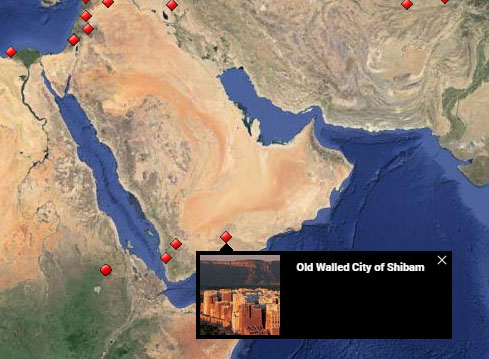
\includegraphics{unesco_map.jpg}}
			\end{center}
		\end{figure}
		\vspace{1cm}
	\end{column}
	\end{columns}
\end{frame}

% Slide 2
\section{Vznik}
\begin{frame}{\textsc{Vznik mesta}}
\transwipe
	\begin{itemize}
	\item Utečenci založili okolo roku $250$ n.l.
	\item Bolo postavených okolo $500$ obytných domov
	\item Domy stavali len z~hlinených tehál
	\item Dodnes stavitelia pracujú podľa tradícii predkov
	\end{itemize}
	\begin{figure}[ht]
		\begin{center}
			\scalebox{0.325}{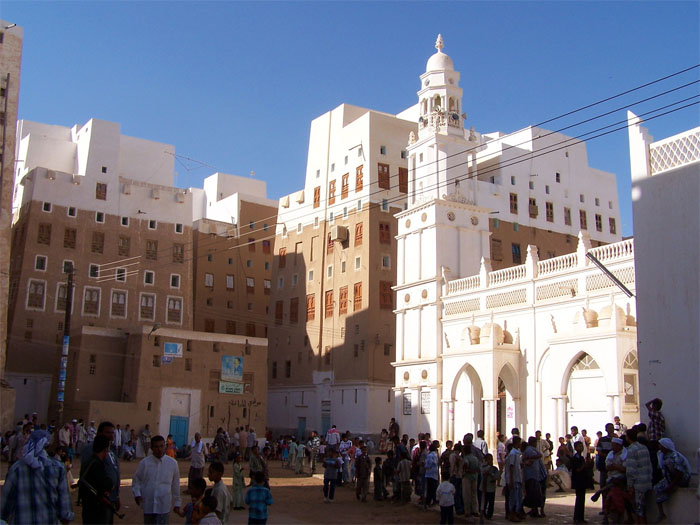
\includegraphics{shi4.jpg}}
		\end{center}
	\end{figure}
\end{frame}

% Slide 3
\section{Minulosť}
\begin{frame}{\textsc{Jeho minulosť (1/2)}}
\transwipe
	\begin{itemize}
	\item Rozkvet mesta kvôli karaváne -- Kadidlová cesta
	\item Po nej dopravovali surovú gumu z~kadidlových stromov
		\begin{itemize}
		\item[•] horenie gumy vytvára silnú vôňu so silnou arómou
		\item[•] používa sa dodnes v~kadidlách {\scriptsize (Egypt, Grécko, židovké chrámy)}
		\end{itemize}
	\end{itemize}
	\begin{figure}[ht]
		\begin{center}
			\scalebox{0.3}{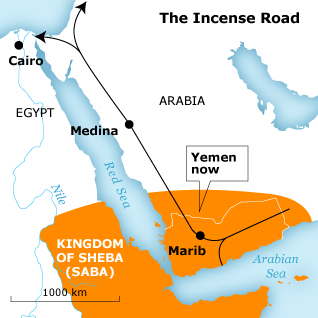
\includegraphics{road_map.jpg}} \scalebox{0.27}{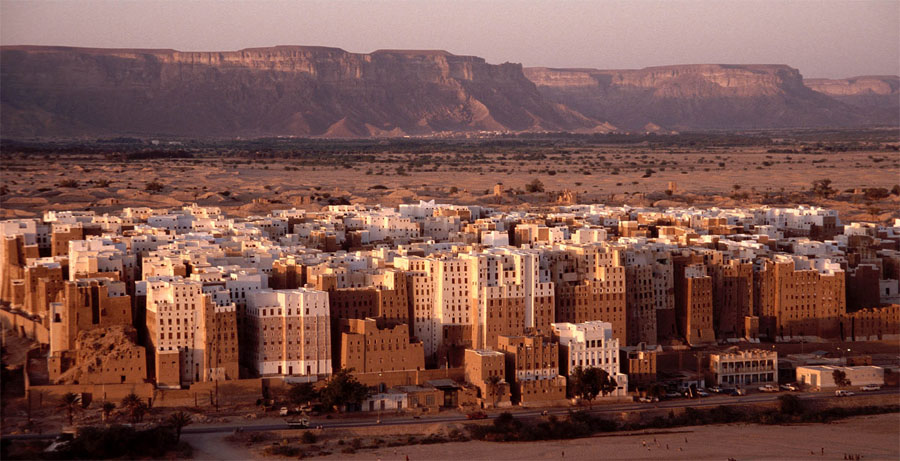
\includegraphics{shi2.jpg}}
		\end{center}
	\end{figure}
\end{frame}

% Slide 4	
\begin{frame}{\textsc{Minulosť (2/2)}}
\transwipe
	\begin{itemize}
	\item Okrem kadidlovej gumy sa dopravovali ďalšie suroviny
		\begin{itemize}
		\item[•] zlato, tkaniny, korenie, drahé kamene
		\end{itemize}
	\item Koniec rozkvetu v~9.st., kvôli strate významu Kadidlovej cesty
	\item Odvtedy ostala architektonická tvár bezo zmeny
	\end{itemize}
	\bigskip
	\begin{figure}[ht]
		\begin{center}
			\scalebox{0.5}{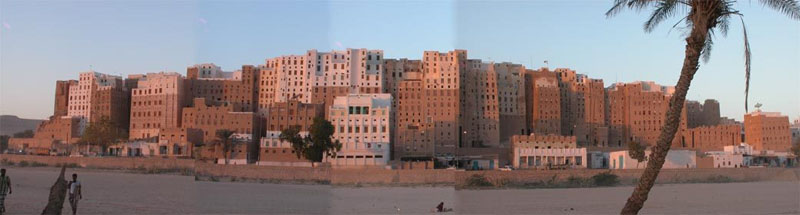
\includegraphics{shi5.jpg}}
		\end{center}
	\end{figure}
\end{frame}

% Slide 5
\section{Vzhľad}
\begin{frame}{\textsc{Vzhľad}}
\transwipe
	\begin{itemize}
	\item Mrakodrapy tehlovej farby alebo natreté vápnom
	\item Vysoké okolo 30 metrov, až do 8 poschodí
	\item Často zdobené prekrásnymi vyrezávanými bránami
	\item Obklopený múrom, slúžiacim ako protipovodňová bariéra
	\item Po záplavách v~roku 1532 bola väčšina budov opravovaná
	\end{itemize}
	\begin{figure}[ht]
		\begin{center}
			\scalebox{0.35}{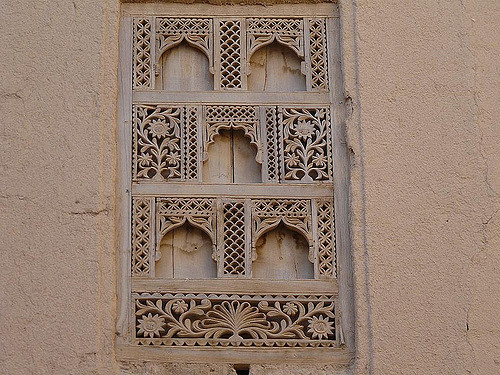
\includegraphics{window.jpg}}\hspace{1cm} \scalebox{0.41}{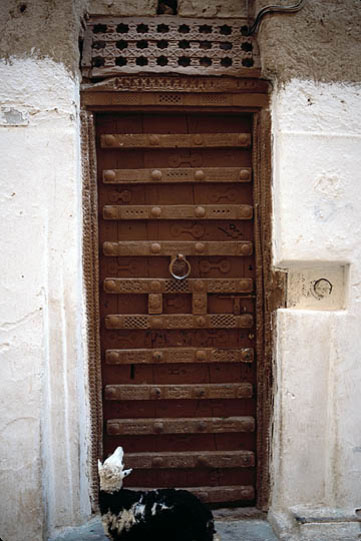
\includegraphics{door2.jpg}}
		\end{center}
	\end{figure}
\end{frame}

% Slide 6
\section{Súčasnosť}
\begin{frame}{\textsc{Súčasnosť -- Mesto v~ohrození}}
\transwipe
	\begin{itemize}
	\item Roku $1982$ pridané do svetového dedičstva \textsc{UNESCO}\\
		a~v~roku $2015$ pripísaný do svetového dedičstva v~ohrození
	\item Dnes okolo $7\,000$ obyvateľov
	\item Budovy začínajú chátrať
	\end{itemize}
	\begin{figure}[ht]
		\begin{center}
			\scalebox{0.225}{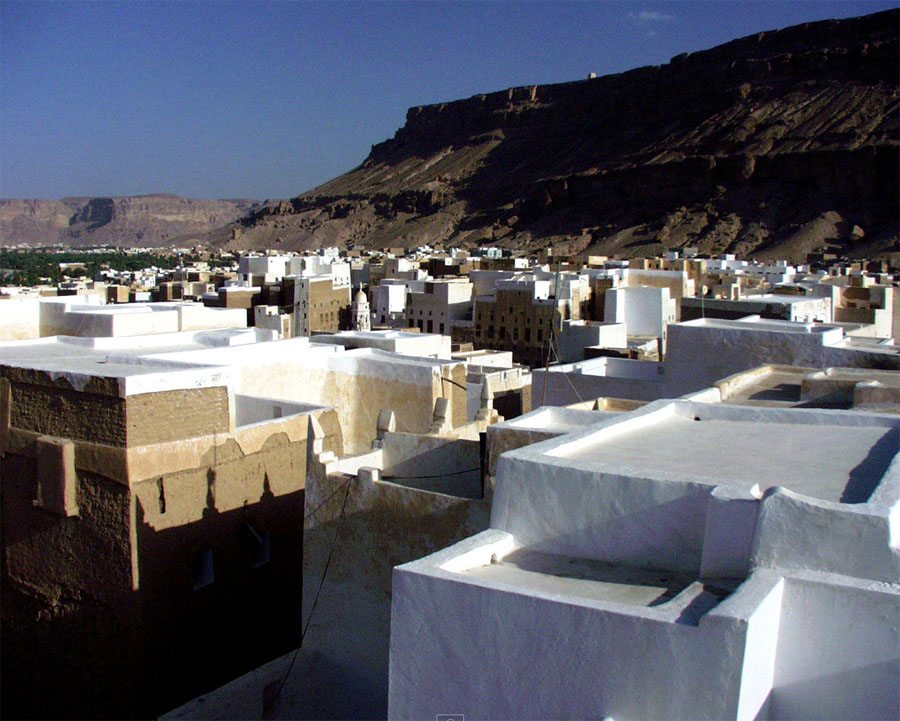
\includegraphics{shi3.jpg}}
		\end{center}
	\end{figure}
\end{frame}

% Slide Zdroje
\section{Zdroje}
%	Cite: Wikipedia. "Shibam" [online]. Posledná zmena 28 júla 2015 [cit. 2016-04-26]. Dostupné na: {https://en.wikipedia.org/wiki/Shibam}.
%	Cite: UNESCO. "Old Walled City of Shibam" [online]. [cit. 2016-04-26]. Dostupné na: {http://whc.unesco.org/en/list/192}.
%	“Old Walled City of Shibam.” – UNESCO World Heritage Centre. N.p., n.d. Web. 2011/ 15 Nov. 2015.
%	Cite: Finn MacLeod. "The 'Manhattan of the Desert': Shibam, Yemen's Ancient Skyscraper City" 02 Aug 2015. ArchDaily. Accessed 26 Apr 2016. <http://www.archdaily.com/771154/the-manhattan-of-the-desert-shibam-yemens-ancient-skyscraper-city/>
\begin{frame}{\textsc{Použité zdroje}}
\transdissolve
	\footnotesize
	\begin{itemize}
	\item {{\textsc{UNESCO World Heritage Centre}}}: \emph{Old Walled City of Shibam} 2011. {\scriptsize[cit. 2016-04-26]}\\
		\texttt{http://whc.unesco.org/en/list/192}
	\item {{\textsc{Finn MacLeod}}}: \emph{The 'Manhattan of the Desert': Shibam, Yemen's Ancient Skyscraper City}  02 Aug 2015. ArchDaily. {\scriptsize[cit. 2016-04-26]}\\
		\texttt{http://www.archdaily.com/771154/the-manhattan-of-the-desert-shibam-yemens-ancient-skyscraper-city}
	\item {{\textsc{Wikipedia}}}: \emph{Shibam} 28 July 2015. {\scriptsize[cit. 2016-04-26]}\\
		\texttt{https://en.wikipedia.org/wiki/Shibam}
	\item[Príloha:] {{\textsc{Augustín, M}}}. \emph{SHIBAM} {\scriptsize[word dokument]}. B.~Bystrica: GJGT, 2012.\\
		{\scriptsize Poznámka: stratené zdroje pre tento dokument; hrubý text.}
	\end{itemize}
\end{frame}
\end{document}
